%Chapter 2
\chapter{Literature study}
\thispagestyle{empty}
\vspace{38em}
\hrulefill
\\
\enquote*{\textit{Quote.}} - Somebody\\
\newpage
\section{Introduction}
\section{Methods to identify operational improvements}
	\subsection{Preamble}
	\subsection{Identifying areas for improvement}
		(Kriel Masters)
		-Investigation\\
		-Measurements\\
		-Simulated impact of the proposed intervention\\
	\subsection{Measurements}	
	\subsection{Leakage detection}
		(Van Tonder masters)
		- Inspections\\
		- Audible sounds (by ear)\\
		- Ultrasonic\\
		- Intelligent leakage detection (instrumentaion SCADA)\\
		- Alternatives (pigging, soap water, Dyes load/unload test)\\
		-  CALDS ( Compressed air leakage document system)\\

	\subsection{Estimation techniques}
		- Snyman estimated improvements using historical data.\cite{Snyman2011Masters}\\
		- Marais estimation through simplified estimation, simulation \cite{Marais2012PhD, marais2013simplification}.

	\subsection{Summary}
\section{Review of compressed air energy interventions in industry}
	\subsection{Preamble}
	(Kriel Masters)
	- Supply and demand strategies (improving compressor efficiency vs reducing/improving demand)\\
	Marais et al investigated increased energy savings through the use of \gls{calds} \cite{marais2009increased}.
	\subsection{Strategies to improve compressed air supply}
		- Control Strategies\\
		- Relocating compressor. reconfiguring networks - Bredenkamp\\
		- Compressor schedules\\
		- Variable speed drives\\
		- Compressor selection\\
		- Marais showed compressed air saving potential through an expert control 	system.\cite{marais2010expert}\\
	\subsection{Strategies to reduce/optimise compressed air consumption}
		- Reducing leaks\\
		- Control Valves - Pascoe\\
		- Marais PhD\\
\\
		- Snyman - investigated various Compressed air demand reduction and efficiency optimisations \cite{Snyman2011Masters}.
		\paragraph{Pneumatic rock drills efficiency}\leavevmode\\
		Reduced pressure to the drill will cause it to run even less efficiently. A study by  Bester \textit{et al.} showed that between 2002 and 2013 compressed air and energy consumption per tonne of ore produced had steadily increased as shown in figure \ref{fig: Compressed energy and air flow per ton}. The increase in consumption per \gls{t} was a result of a reduction in air pressure at the mining stopes. Measurements indicated that the pressure was as low as 300 \gls{kpa}. This reduced the efficiency of the rock drills. Before 2002 pressure was maintained above 500 \gls{kpa} at the stopes.  .\cite{bester2013effect} \par
		\begin{figure}[h]
			\centering
			\fbox{% GNUPLOT: LaTeX picture with Postscript
\begingroup
  \makeatletter
  \providecommand\color[2][]{%
    \GenericError{(gnuplot) \space\space\space\@spaces}{%
      Package color not loaded in conjunction with
      terminal option `colourtext'%
    }{See the gnuplot documentation for explanation.%
    }{Either use 'blacktext' in gnuplot or load the package
      color.sty in LaTeX.}%
    \renewcommand\color[2][]{}%
  }%
  \providecommand\includegraphics[2][]{%
    \GenericError{(gnuplot) \space\space\space\@spaces}{%
      Package graphicx or graphics not loaded%
    }{See the gnuplot documentation for explanation.%
    }{The gnuplot epslatex terminal needs graphicx.sty or graphics.sty.}%
    \renewcommand\includegraphics[2][]{}%
  }%
  \providecommand\rotatebox[2]{#2}%
  \@ifundefined{ifGPcolor}{%
    \newif\ifGPcolor
    \GPcolortrue
  }{}%
  \@ifundefined{ifGPblacktext}{%
    \newif\ifGPblacktext
    \GPblacktextfalse
  }{}%
  % define a \g@addto@macro without @ in the name:
  \let\gplgaddtomacro\g@addto@macro
  % define empty templates for all commands taking text:
  \gdef\gplbacktext{}%
  \gdef\gplfronttext{}%
  \makeatother
  \ifGPblacktext
    % no textcolor at all
    \def\colorrgb#1{}%
    \def\colorgray#1{}%
  \else
    % gray or color?
    \ifGPcolor
      \def\colorrgb#1{\color[rgb]{#1}}%
      \def\colorgray#1{\color[gray]{#1}}%
      \expandafter\def\csname LTw\endcsname{\color{white}}%
      \expandafter\def\csname LTb\endcsname{\color{black}}%
      \expandafter\def\csname LTa\endcsname{\color{black}}%
      \expandafter\def\csname LT0\endcsname{\color[rgb]{1,0,0}}%
      \expandafter\def\csname LT1\endcsname{\color[rgb]{0,1,0}}%
      \expandafter\def\csname LT2\endcsname{\color[rgb]{0,0,1}}%
      \expandafter\def\csname LT3\endcsname{\color[rgb]{1,0,1}}%
      \expandafter\def\csname LT4\endcsname{\color[rgb]{0,1,1}}%
      \expandafter\def\csname LT5\endcsname{\color[rgb]{1,1,0}}%
      \expandafter\def\csname LT6\endcsname{\color[rgb]{0,0,0}}%
      \expandafter\def\csname LT7\endcsname{\color[rgb]{1,0.3,0}}%
      \expandafter\def\csname LT8\endcsname{\color[rgb]{0.5,0.5,0.5}}%
    \else
      % gray
      \def\colorrgb#1{\color{black}}%
      \def\colorgray#1{\color[gray]{#1}}%
      \expandafter\def\csname LTw\endcsname{\color{white}}%
      \expandafter\def\csname LTb\endcsname{\color{black}}%
      \expandafter\def\csname LTa\endcsname{\color{black}}%
      \expandafter\def\csname LT0\endcsname{\color{black}}%
      \expandafter\def\csname LT1\endcsname{\color{black}}%
      \expandafter\def\csname LT2\endcsname{\color{black}}%
      \expandafter\def\csname LT3\endcsname{\color{black}}%
      \expandafter\def\csname LT4\endcsname{\color{black}}%
      \expandafter\def\csname LT5\endcsname{\color{black}}%
      \expandafter\def\csname LT6\endcsname{\color{black}}%
      \expandafter\def\csname LT7\endcsname{\color{black}}%
      \expandafter\def\csname LT8\endcsname{\color{black}}%
    \fi
  \fi
    \setlength{\unitlength}{0.0500bp}%
    \ifx\gptboxheight\undefined%
      \newlength{\gptboxheight}%
      \newlength{\gptboxwidth}%
      \newsavebox{\gptboxtext}%
    \fi%
    \setlength{\fboxrule}{0.5pt}%
    \setlength{\fboxsep}{1pt}%
\begin{picture}(9360.00,4032.00)%
    \gplgaddtomacro\gplbacktext{%
      \colorrgb{0.42,0.42,0.42}%
      \put(682,924){\makebox(0,0)[r]{\strut{}$0$}}%
      \colorrgb{0.42,0.42,0.42}%
      \put(682,1230){\makebox(0,0)[r]{\strut{}$5$}}%
      \colorrgb{0.42,0.42,0.42}%
      \put(682,1536){\makebox(0,0)[r]{\strut{}$10$}}%
      \colorrgb{0.42,0.42,0.42}%
      \put(682,1842){\makebox(0,0)[r]{\strut{}$15$}}%
      \colorrgb{0.42,0.42,0.42}%
      \put(682,2148){\makebox(0,0)[r]{\strut{}$20$}}%
      \colorrgb{0.42,0.42,0.42}%
      \put(682,2453){\makebox(0,0)[r]{\strut{}$25$}}%
      \colorrgb{0.42,0.42,0.42}%
      \put(682,2759){\makebox(0,0)[r]{\strut{}$30$}}%
      \colorrgb{0.42,0.42,0.42}%
      \put(682,3065){\makebox(0,0)[r]{\strut{}$35$}}%
      \colorrgb{0.42,0.42,0.42}%
      \put(682,3371){\makebox(0,0)[r]{\strut{}$40$}}%
      \colorrgb{0.42,0.42,0.42}%
      \put(814,704){\makebox(0,0){\strut{}$2002$}}%
      \colorrgb{0.42,0.42,0.42}%
      \put(2025,704){\makebox(0,0){\strut{}$2004$}}%
      \colorrgb{0.42,0.42,0.42}%
      \put(3237,704){\makebox(0,0){\strut{}$2006$}}%
      \colorrgb{0.42,0.42,0.42}%
      \put(4448,704){\makebox(0,0){\strut{}$2008$}}%
      \colorrgb{0.42,0.42,0.42}%
      \put(5659,704){\makebox(0,0){\strut{}$2010$}}%
      \colorrgb{0.42,0.42,0.42}%
      \put(6871,704){\makebox(0,0){\strut{}$2012$}}%
      \colorrgb{0.42,0.42,0.42}%
      \put(8082,704){\makebox(0,0){\strut{}$2014$}}%
      \colorrgb{0.42,0.42,0.42}%
      \put(8214,924){\makebox(0,0)[l]{\strut{}$0$}}%
      \colorrgb{0.42,0.42,0.42}%
      \put(8214,1230){\makebox(0,0)[l]{\strut{}$50$}}%
      \colorrgb{0.42,0.42,0.42}%
      \put(8214,1536){\makebox(0,0)[l]{\strut{}$100$}}%
      \colorrgb{0.42,0.42,0.42}%
      \put(8214,1842){\makebox(0,0)[l]{\strut{}$150$}}%
      \colorrgb{0.42,0.42,0.42}%
      \put(8214,2148){\makebox(0,0)[l]{\strut{}$200$}}%
      \colorrgb{0.42,0.42,0.42}%
      \put(8214,2453){\makebox(0,0)[l]{\strut{}$250$}}%
      \colorrgb{0.42,0.42,0.42}%
      \put(8214,2759){\makebox(0,0)[l]{\strut{}$300$}}%
      \colorrgb{0.42,0.42,0.42}%
      \put(8214,3065){\makebox(0,0)[l]{\strut{}$350$}}%
      \colorrgb{0.42,0.42,0.42}%
      \put(8214,3371){\makebox(0,0)[l]{\strut{}$400$}}%
    }%
    \gplgaddtomacro\gplfronttext{%
      \csname LTb\endcsname%
      \put(176,2147){\rotatebox{-270}{\makebox(0,0){\strut{}kWh/t}}}%
      \put(8851,2147){\rotatebox{-270}{\makebox(0,0){\strut{}$m^3$/t}}}%
      \put(4448,374){\makebox(0,0){\strut{}Year}}%
      \put(4448,3701){\makebox(0,0){\strut{}Compressed air energy and Volume consumed per ton}}%
      \csname LTb\endcsname%
      \put(3593,173){\makebox(0,0)[r]{\strut{}Energy per Ton (kWh/t)}}%
      \csname LTb\endcsname%
      \put(7352,173){\makebox(0,0)[r]{\strut{}Volume per Ton ($m^3$/t)}}%
    }%
    \gplbacktext
    \put(0,0){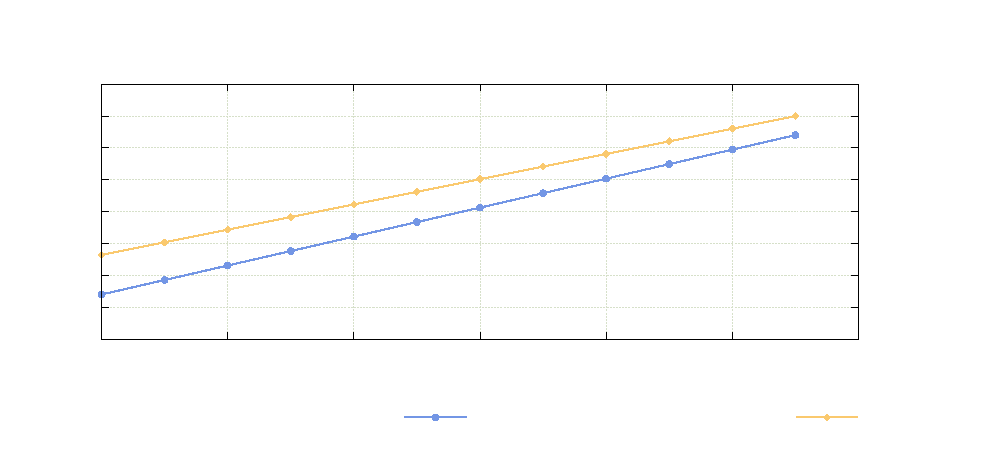
\includegraphics{Graphs/1/EVperT/EVperT}}%
    \gplfronttext
  \end{picture}%
\endgroup
}
			\caption[The Compressed air energy and flow consumed per T of ore produced.]{The Compressed air energy and flow consumed per T of ore produced. Adopted from Bester \textit{et al.} \cite{bester2013effect}.}
			\label{fig: Compressed energy and air flow per ton}
		\end{figure}
	\subsection{Summary}
\section{Use of simulations to identify improvements in mining systems}
	\subsection{Preamble}
	\subsection{Value of simulation in DSM projects}
		(Van Niekerk M)\\
		- Compressed air \\
		- Cooling systems\\
		- Dewatering\\
		- Design optimisations using simulation\\
 		- KYPipe’s gas simulation engine\\
		- De Coning -  simulations to investigate the opportunity to optimise the control strategy of a compressed air network by rescheduling the compressors.
	\subsection{Simulation procedures}
		-Kriel masters\\
		-Pascoe\\
		\paragraph{Periodic simulation}\leavevmode\\
 	\subsection{Verifying simulations}
 		- Holman
 		- van Niekerk masters\\
 		- Kriel masters ( validation)\\
 		- Calibrating -pascoe
 		- determining accuracy - pascoe
 		- Du2015Development
 		- comparisons with models
 		- comparison with actual 
 		- First principles
 	\subsection{Shortcoming of previous studies}
	\subsection{Summary}
\section{Conclusion}